\documentclass[a4paper,USenglish,cleveref, autoref]{lipics-v2019}
%This is a template for producing LIPIcs articles.
%See lipics-manual.pdf for further information.
%for A4 paper format use option "a4paper", for US-letter use option "letterpaper"
%for british hyphenation rules use option "UKenglish", for american hyphenation rules use option "USenglish"
%for section-numbered lemmas etc., use "numberwithinsect"
%for enabling cleveref support, use "cleveref"
%for enabling cleveref support, use "autoref"

\bibliographystyle{plainurl}% the mandatory bibstyle

\usepackage{enumerate} % for lists
\usepackage{listings} % for code
\usepackage{xspace} % so we don't need to figure out spacing after \toolname every time
\usepackage{mathpartir} % for inference rules
\usepackage{scalerel} % to render definitional equality
\usepackage{bbm} % to render N for the natural numbers
\usepackage{syntax} % for code highlighting
\usepackage{xcolor} % for code highlighting
\usepackage{multirow} % for tables

\nolinenumbers % it's impossible to get this to look reasonable with inline code

% Nice rendering of Coq code
\lstdefinelanguage{coq}{
    keywords={Theorem, Proof, Record, Lemma, Definition, Abort, Qed, forall, Inductive, Type, Prop, Set, fun, fix, forall, Require, Import, Fixpoint, match, end, with, in, as, return, struct, Qed, Defined, let},
    basicstyle=\linespread{0.95}\small\ttfamily,
    keywordstyle=\color{blue},
    commentstyle=\itshape\rmfamily,
    showstringspaces=false,
    columns=flexible,
    breaklines=true,
    texcl=true,
    mathescape=true,
    tabsize=4,
    stringstyle=\color{brown},
    escapeinside={(@}{@)},
}

\lstset{language=coq} % default

\title{Ornaments for Proof Reuse in Coq}
%\subtitle{Subtitle Text, if any}

\titlerunning{}%optional, please use if title is longer than one line

\author{Talia Ringer}{University of Washington, USA}{tringer@cs.washington.edu}{}{}

\author{Nathaniel Yazdani}{University of Washington, USA}{nyazdani@cs.washington.edu}{}{}

\author{John Leo}{Halfaya Research}{leo@halfaya.org}{}{}

\author{Dan Grossman}{University of Washington, USA}{djg@cs.washington.edu}{}{}

\authorrunning{T. Ringer, N. Yazdani, J. Leo, and D. Grossman}%mandatory. First: Use abbreviated first/middle names. Second (only in severe cases): Use first author plus 'et al.'

\Copyright{Talia Ringer, Nathaniel Yazdani, John Leo, and Dan Grossman}%mandatory, please use full first names. LIPIcs license is "CC-BY";  http://creativecommons.org/licenses/by/3.0/

\ccsdesc[500]{Software and its engineering~Formal software verification}

\keywords{ornaments, proof reuse, proof automation}

\category{}%optional, e.g. invited paper

\relatedversion{}%optional, e.g. full version hosted on arXiv, HAL, or other respository/website
%\relatedversion{A full version of the paper is available at \url{...}.}

\supplement{The Coq plugin, examples, and case study code for this paper can be found at \url{http://github.com/uwplse/ornamental-search/tree/itp+equiv}}
\label{supplement}
%optional, e.g. related research data, source code, ... hosted on a repository like zenodo, figshare, GitHub, ...

\EventEditors{John Harrison, John O'Leary, and Andrew Tolmach}
\EventNoEds{3}
\EventLongTitle{10th International Conference on Interactive Theorem Proving (ITP 2019)}
\EventShortTitle{ITP 2019}
\EventAcronym{ITP}
\EventYear{2019}
\EventDate{September 9--12, 2019}
\EventLocation{Portland, OR, USA}
\EventLogo{}
\SeriesVolume{141}
\ArticleNo{4}

\begin{document}

% https://tex.stackexchange.com/questions/4216/how-to-typeset-correctly
\newcommand\defeq{\equiv_{\scaleto{\beta\delta\iota}{4pt}}} % definitional equality
\newcommand{\smallmath}[1]{$\text{\small #1}$} % inline math looks terrible at normal size
\newcommand\A{\smallmath{$A$}} % recurring type A
\newcommand\B{\smallmath{$B$}} % recurring type B
\newcommand\IB{\smallmath{$I_B$}} % recurring type I_B
\newcommand\sigT{\smallmath{$\Sigma$}} % sigma types
\newcommand\exT{\smallmath{$\exists$}} % existentials
\newcommand\Pil{\smallmath{$\pi_l$}} % left projection
\newcommand\Pir{\smallmath{$\pi_r$}} % right projection
\newcommand\toolname{\textsc{Devoid}\xspace} % DEVOID tool name
\newcommand{\reducedstrut}{\vrule width 0pt height .9\ht\strutbox depth .9\dp\strutbox\relax} % for \codediff and \codeauto
\newcommand{\codediff}[1]{%
  \begingroup
  \setlength{\fboxsep}{0pt}%
  \colorbox{orange!25}{\reducedstrut#1\/}%
  \endgroup
} % to highlight the difference between two code blocks
\newcommand{\codeauto}[1]{%
  \begingroup
  \setlength{\fboxsep}{0pt}%
  \colorbox{cyan!30}{\reducedstrut#1\/}%
  \endgroup
} % to highlight automatically-generated terms

\maketitle

\begin{abstract}
Ornaments express relations between inductive types with the same inductive structure.
We implement fully automatic proof reuse for a particular class of ornaments in a Coq plugin,
and show how such a tool can give programmers the rewards of using indexed inductive types
while automating away many of the costs.
The plugin works directly on Coq code; it is the first ornamentation tool for a
non-embedded dependently typed language.
It is also the first tool to automatically identify ornaments:
To lift a function or proof,
the user must provide only the source type, the destination type, and the source function or proof.
In taking advantage of the mathematical properties of ornaments, our approach produces faster functions and smaller terms 
than a more general approach to proof reuse in Coq.
\end{abstract}

\section{Introduction}

%Proof assistants allow programmers to verify everything from distributed systems~\cite{wilcox:verdi} and compilers~\cite{leroy:compcert} to
%formalizations of mathematics~\cite{DBLP:journals/corr/BauerGLSSS16}. 

Proof automation makes verification more accessible to programmers, but it is often intractable
without programmer guidance. In \textit{interactive theorem proving} (ITP), the programmer guides the 
proof search process. The guidance reduces the search space to make proof automation more tractable.
This in turns helps the programmer, who does not have to manually verify the entire system.

%Interactive theorem provers allow programmers to guide proof search and interactively 
%verify everything from distributed systems~\cite{wilcox:verdi} and compilers~\cite{leroy:compcert} to
%formalizations of mathematics~\cite{DBLP:journals/corr/BauerGLSSS16}. In many of these theorem provers, programmers use

%In these languages, programmers write precise specifications of programs
%and prove implementations correct with respect to the specifications.

Despite automation, programming in these proof assistants is brittle: Even a minor change to a definition or theorem
can break many dependent proofs. This is a major source of development inefficiency in proof assistants
based on dependent type theory~\cite{proof-eng, Aydemir2008, Delaware2013ICFP}.

Traditional proof automation does not consider how proofs, definitions, and theorems change over time.
Instead, it is driven by the state of the current proof, sometimes with supplementary
information from other proofs, definitions, and theorems (as in hint databases~\cite{hints} and rippling~\cite{rippling}).
This puts the burden of dealing with brittleness on the programmer. 

We present a new approach to proof automation that accounts for breaking changes. %:
%searching the difference in versions of a proof, definition, or theorem. 
%We reimagine the problem of proof reuse~\cite{Boite2004, Mulhern06proofweaving} 
%in the context of traditional automation for ITP. 
In our approach, the programmer guides proof search 
by providing an \textit{example} of how to adapt proofs to changes in definitions or theorems.
A tool then generalizes the example adaptation into a \textit{reusable patch} that the programmer can use to fix
other broken proofs.

In doing so, we chart a path for a future %of ITP 
that moves the burden of brittleness
away from the programmer and into proof automation. 
Programmers typically address brittleness through design principles that make proofs
resilient to change~\cite{proof-eng, Aydemir2008, Delaware2013ICFP}, or through program-specific proof automation~\cite{chlipala:cpdt}.
These techniques, while useful, have limitations: 
Planning a verification effort around future change is challenging, and program-specific automation requires specialized knowledge.
The programmer's ability to anticipate likely changes determines the robustness of both techniques in
the face of change. %The robustness of both techniques in the face of change is determined by the programmer's ability to anticipate likely changes. 
Even then, many breaking changes are outside of the programmer's control. Updating proof assistant
versions, for example, can break proofs regardless of planning or automation~\cite{verdicommit}.

\begin{figure*}[ht]
\begin{minipage}{0.48\textwidth}
\centering
\lstset{language=coq, aboveskip=0pt, belowskip=0pt}
\lstinputlisting[firstline=1, lastline=3]{repair/izr.tex}
\lstinputlisting[backgroundcolor=\color{orange!35},firstline=4,lastline=5]{repair/izr.tex}
\lstinputlisting[firstline=6, lastline=6]{repair/izr.tex}
\end{minipage}
\hfill
\begin{minipage}{0.48\textwidth}
\centering
\lstset{language=coq, aboveskip=0pt, belowskip=0pt}
\lstinputlisting[firstline=8, lastline=10]{repair/izr.tex}
\lstinputlisting[backgroundcolor=\color{orange!35},firstline=11,lastline=12]{repair/izr.tex}
\lstinputlisting[firstline=13, lastline=13]{repair/izr.tex}
\end{minipage}
\vspace{-.3cm}
%\setlength{\belowcaptionskip}{-2pt}
\caption[Caption]{Old (left) and new (right) definitions of \lstinline{IZR} in Coq.
The old definition applies injection from naturals to reals and conversion of positives to
naturals; the new definition applies injection from positives to reals.}
\label{fig:izr}
\end{figure*}


We identify a set of core components that are critical to searching an example for patches in Coq.
We use the components to build %four different 
a procedure for finding patches %for non-structural changes 
in a Coq plugin as a 
proof-of-concept.
Case studies on real projects like CompCert~\cite{leroy:compcert} and the Coq standard library
suggest that patches are useful for realistic scenarios, and that it is simple to compose the components 
to handle different classes of changes.
We test the boundaries of the components on a suite of tests
and show how our findings can help build the future we envision.

In summary, we contribute the following:

\begin{enumerate}
%\item We develop new foundations for proof automation in ITP that account for breaking changes. % TODO reword
\item We identify a set of core components that are key to searching for patches.
\item We demonstrate that these core components are useful on real changes in Coq code.
\item We explore how to drive a future that moves the burden of change in ITP away from the programmer and into automated tooling.
\end{enumerate}

% TODO fix contributions

% evaluation stuff in contributions too

% SOMEWHERE: we focus on non-structural changes





\section{Motivating Example: Porting a Library}
\label{sec:example}

\toolnameb is a plugin for Coq 8.8; it can be found in the repository linked to as \textbf{Supplement Material} under the abstract of this paper.
To see how it works, consider an example using the types from Figure~\ref{fig:listvect},
the code for which is in \href{http://github.com/uwplse/ornamental-search/blob/itp+equiv/plugin/coq/examples/Example.v}{\lstinline{Example.v}}.
In this example, we lift two list zip functions and a proof of a theorem relating them from the Haskell CoreSpec library~\cite{hstocoqv}:
\begin{lstlisting}
zip {T$_1$ T$_2$}: list T$_1$ $\rightarrow$ list T$_2$ $\rightarrow$ list (T$_1$ * T$_2$).
zip_with {T$_1$ T$_2$ T$_3$} (f : T$_1$ $\rightarrow$ T$_2$ $\rightarrow$ T$_3$): list T$_1$ $\rightarrow$ list T$_2$ $\rightarrow$ list T$_3$.
zip_with_is_zip {T$_1$ T$_2$}: $\forall$(l$_1$:list T$_1$)(l$_2$:list T$_2$), zip_with pair l$_1$ l$_2$ = zip l$_1$ l$_2$.
\end{lstlisting}
\toolnameb runs a preprocessing step before lifting, which we describe in Section~\ref{sec:impl}; we assume this step has already run.
We use the \codeauto{cyan} background color to denote tool-produced terms and the names that refer to them.
We run \toolnameb to lift functions and proofs from lists to vectors, but it can also lift in the opposite direction.

\subparagraph*{Step 1: Search.}
We first use \toolnameb's \lstinline{Find ornament} command to search for the relation between lists and vectors:
\begin{lstlisting}
Find ornament list vector.
\end{lstlisting}
This produces functions which together form an equivalence (denoted \smallmath{$\simeq$}):
\begin{lstlisting}
list T $\simeq$ $\Sigma$ (n : nat).vector T n
\end{lstlisting}

\subparagraph*{Step 2: Lift.}
We then lift our functions and proofs
along that equivalence using \toolnameb's \lstinline{Lift} command.
For example, to lift \lstinline{zip}, we run the command:
\begin{lstlisting}
Lift list vector in zip as (@\codeauto{zipV\_p}@).
\end{lstlisting}
This produces a function with this type:
\begin{lstlisting}
(@\codeauto{zipV\_p}@) {T$_1$ T$_2$} : $\Sigma$ n.vector T$_1$ n $\rightarrow$ $\Sigma$ n.vector T$_2$ n $\rightarrow$ $\Sigma$ n.vector (T$_1$ * T$_2$) n.
\end{lstlisting}
that behaves like \lstinline{zip}, but whose body no longer refers to lists.
We lift our proof similarly:
\begin{lstlisting}
Lift list vector in zip_with_is_zip as (@\codeauto{zip\_with\_is\_zipV\_p}@).
\end{lstlisting}
This produces a proof of the analogous result (denoting projections by \smallmath{$\pi_{l}$} and \smallmath{$\pi_{r}$}):
\begin{lstlisting}
(@\codeauto{zip\_with\_is\_zipV\_p}@) {T$_1$ T$_2$} : $\forall$ (v$_1$ : $\Sigma$ n.vector T$_1$ n) (v$_2$ : $\Sigma$ n.vector T$_2$ n),
  (@\codeauto{zip\_withV\_p}@) pair ($\exists$ ($\pi_l$ v$_1$) ($\pi_r$ v$_1$)) ($\exists$ ($\pi_l$ v$_2$) ($\pi_r$ v$_2$)) =
  (@\codeauto{zipV\_p} ($\exists$ ($\pi_l$ v$_1$) ($\pi_r$ v$_1$)) ($\exists$ ($\pi_l$ v$_2$) ($\pi_r$ v$_2$)).
\end{lstlisting}
that no longer refers to lists, \lstinline{zip}, or \lstinline{zip_with} in any way.

\subparagraph*{Step 3: Unpack.}
The lifted terms operate over vectors whose lengths are \textit{packed} inside of a sigma type.
While this lets \lstinline{Lift} provide strong theoretical guarantees, it can make it difficult to interface with the lifted code.
We can recover \textit{unpacked} terms using \toolnameb's \lstinline{Unpack} command.
For example, to unpack \codeauto{\lstinline{zipV_p}}, we run the command:
\begin{lstlisting}
Unpack $\codeauto{zipV\_p}$ as $\codeauto{zipV}$.
\end{lstlisting}
This produces functions and proofs that operate directly over vectors, like \codeauto{\lstinline{zipV}}:
\begin{lstlisting}
(@\codeauto{zipV}@) {T$_1$ T$_2$} {n$_1$} (v$_1$ : vector T$_1$ n$_1$) {n$_2$} (v$_2$ : vector T$_2$ n$_2$) : 
  vector (T$_1$ * T$_2$) ($\pi_l$ ((@\codeauto{zipV\_p}@) ($\exists$ n$_1$ v$_1$) ($\exists$ n$_2$ v$_2$))).
\end{lstlisting}
and \codeauto{\lstinline{zip\_with\_is\_zipV}}:
\begin{lstlisting}
(@\codeauto{zip\_with\_is\_zipV}@) : $\forall$ {T$_1$ T$_2$} {n$_1$} (v$_1$ : vector T$_1$ n$_1$) {n$_2$} (v$_2$ : vector T$_2$ n$_2$),
  eq_dep _ _ _ ((@\codeauto{zip\_withV}@) pair v$_1$ v$_2$) _ ((@\codeauto{zipV}@) v$_1$ v$_2$).
\end{lstlisting}

\subparagraph*{Step 4: Interface.}
For any two inputs of the same length, \codeauto{\lstinline{zipV}} and \codeauto{\lstinline{zipV_with}} contain proofs
that the output has the same length as the inputs.
However, the types obscure this information.
\href{http://github.com/uwplse/ornamental-search/blob/itp+equiv/plugin/coq/examples/Example.v}{\lstinline{Example.v}} explains how to recover more user-friendly types, like that of \lstinline{zipV_uf}:
\begin{lstlisting}
zipV_uf {T$_1$ T$_2$} {n} : vector T$_1$ n $\rightarrow$ vector T$_2$ n $\rightarrow$ vector (T$_1$ * T$_2$) n.
\end{lstlisting}
and that of \lstinline{zip_withV_uf}:
\begin{lstlisting}
zip_withV_uf {T$_1$ T$_2$ T$_3$} (f : T$_1$ $\rightarrow$ T$_2$ $\rightarrow$ T$_3$) {n} : 
  vector T$_1$ n $\rightarrow$ vector T$_2$ n $\rightarrow$ vector T$_3$ n.
\end{lstlisting}
which both restrict input lengths.
We can then use our lifted functions and proofs in client code.
For example, we can write a different version of Coq's
\lstinline{BVand} function for bitvectors:
\begin{lstlisting}
BVand {n} (v$_1$ : vector bool n) (v$_2$ : vector bool n) : vector bool n := 
  zip_withV_uf andb v$_1$ v$_2$.
\end{lstlisting}
By working over lists, we are able to reason about only the interesting pieces, thinking about indices only
when relevant; in contrast, when writing proofs over vectors, even simple theorems
can generate tricky proof obligations.
With \toolnameb, the programmer can use the lifted functions and proofs
to interface with code that uses vectors, then switch back to lists when vectors are unmanageable. 
In essence, ornaments form the glue between these types.




\section{Specification}
\label{sec:spec}

This section specifies the two commands that \toolnameb implements:

\begin{enumerate}
\item \lstinline{Find ornament} searches for ornaments (specified in Section~\ref{sec:findspec}, described in Section~\ref{sec:findalg}).
\item \lstinline{Lift} lifts along those ornaments (specified in Section~\ref{sec:liftspec}, described in Section~\ref{sec:liftalg}). 
\end{enumerate}

\subparagraph*{Algebraic Ornaments.}
\toolnameb searches for and lifts along \textit{algebraic ornaments} in particular.
An algebraic ornament relates an inductive type \Aa\ to an indexed version of that type \B\ with a new index of type \IB,
where the new index is fully determined by a unique fold over \Aa. 
For example, \lstinline{vector} is exactly \lstinline{list} with a new index of type \lstinline{nat},
where the new index is fully determined by the \lstinline{length} function. Consequentially, there are two functions:
\begin{lstlisting}
ltv : list T $\phantom{blahblahblahblah}$ $\rightarrow$ $\Sigma$(n : nat).vector T n.
vtl : $\Sigma$(n : nat).vector T n $\rightarrow$ list T.
\end{lstlisting}
that are mutual inverses:
\begin{lstlisting}
$\forall$ (l : list T),$\phantom{blahblahblahblahb}$ vtl (ltv l) = l.
$\forall$ (v : $\Sigma$(n : nat).vector T n), ltv (vtl v) = v.
\end{lstlisting}
and therefore form the type equivalence from Section~\ref{sec:example}.
Moreover, since the new index is fully determined by \lstinline{length}, we can relate \lstinline{length} to \lstinline{ltv}:
\begin{lstlisting}
$\forall$ (l : list T), length l = $\pi_{l}$ (ltv l).
\end{lstlisting}

In general,
we can view an algebraic ornament as a type equivalence: % negative \vspace here is needed to deal with \vec{i}
\begin{lstlisting}
(@\vspace{-0.4cm}@)
$A\ \vec{i}\ \simeq\ \Sigma (n : I_B\ \vec{i}\phantom{_{,}}).B\ (\mathtt{index}\ n\ \vec{i}\phantom{_{,}})$
\end{lstlisting}
where \smallmath{$\vec{i}$} are the indices of \Aa, \IB\ is a function over those indices, 
and the \lstinline{index} operation inserts the new index \smallmath{$n$} at the right offset.
Such a type equivalence consists of two functions~\cite{univalent2013homotopy}:
\begin{lstlisting}
(@\vspace{-0.4cm}@)
promote : $A\ \vec{i}\ \phantom{blahblahblahblahblahbla_{,}} \rightarrow\ \Sigma (n : I_B\ \vec{i}\phantom{_{,}}).B\ (\mathtt{index}\ n\ \vec{i}\phantom{_{,}})$.
(@\vspace{-0.4cm}@)
forget$\phantom{e}$ : $\Sigma (n : I_B\ \vec{i}\phantom{_{,}}).B\ (\mathtt{index}\ n\ \vec{i}\phantom{_{,}})\ \rightarrow\ A\ \vec{i}$.
\end{lstlisting}
that are mutual inverses:\footnote{The adjunction condition follows from section and retraction.}
\begin{lstlisting}
(@\vspace{-0.4cm}@)
section$\phantom{ion}$ : $\forall\ (a : A\ \vec{i}\phantom{_{,}}),\ \phantom{blahblahblahblahblahbla_{,}} $forget$\ ($promote$\ a) \phantom{x} = a$.
(@\vspace{-0.4cm}@)
retraction : $\forall\ (b_{\Sigma} : \Sigma (n : I_B\ \vec{i}\phantom{_{,}}).B\ (\mathtt{index}\ n\ \vec{i}\phantom{_{,}})),\ $promote$\ ($forget$\ b_{\Sigma}) = b_{\Sigma}$.
\end{lstlisting}
An algebraic ornament is additionally equipped with an indexer, which is a unique fold:
\begin{lstlisting}
(@\vspace{-0.4cm}@)
indexer : $A\ \vec{i}\ \rightarrow\ I_B\ \vec{i}$.
\end{lstlisting}
which projects the promoted index:
\begin{lstlisting}
(@\vspace{-0.4cm}@)
coherence : $\forall (a : A\ \vec{i}\phantom{_{,}}),\ $indexer$\ a = \pi_{l}\ ($promote$\ a)$.
\end{lstlisting}
Following existing work~\cite{ko2016programming}, we call this equivalence the \textit{ornamental promotion isomorphism}; 
when it holds and the indexer exists, we say that \B\ is an algebraic ornament of \Aa.

\lstinline{Find ornament} searches for algebraic ornaments between types and is, to the best of our knowledge, the first search algorithm
for ornaments. \lstinline{Lift} then lifts functions and proofs along those ornaments, removing all references to the old type.
Both commands make some additional assumptions for simplicity; detailed explanations for these are
in \href{http://github.com/uwplse/ornamental-search/blob/itp+equiv/plugin/coq/examples/Assumptions.v}{\lstinline{Assumptions.v}}.

\subsection{\lstinline{Find ornament}}
\label{sec:findspec}

In their original form, ornaments are a programming mechanism: Given a type \Aa, an ornament determines
some new type \B. We invert this process for algebraic ornaments: Given types \Aa\ and \B, 
\toolnameb searches for an ornament between them. This is possible for algebraic ornaments precisely because the indexer is extensionally unique.
For example, all possible indexers for \lstinline{list} and \lstinline{vector} must compute
the length of a list; if we were to try doubling the length instead, we would not be able to satisfy the equivalence.

\lstinline{Find ornament} takes two inductive types and searches for the components of the 
ornamental promotion isomorphism between them:

\begin{itemize}
\item \textbf{Inputs}: Inductive types \Aa\ and \B, assuming:
\begin{itemize}
\item \B\ is an algebraic ornament of \Aa,
\item \B\ has the same number of constructors in the same order as \Aa,
\item \Aa\ and \B\ do not contain recursive references to themselves under products, and
\item for every recursive reference to \Aa\ in \Aa, there is exactly one new hypothesis in \B, which is exactly the new index of the corresponding recursive reference in \B.
\end{itemize}
\item \textbf{Outputs}: Functions \lstinline{promote}, \lstinline{forget}, and \lstinline{indexer}, guaranteeing:
\begin{itemize}
\item the outputs form the ornamental promotion isomorphism between the inputs.
\end{itemize}
\end{itemize}

\lstinline{Find ornament} includes an option to generate a proof that the outputs form the ornamental promotion isomorphism;
by default, this option is false, since \lstinline{Lift} does not need this proof.

\subsection{\lstinline{Lift}}
\label{sec:liftspec}

\lstinline{Lift} lifts a term along the ornamental promotion isomorphism between 
\Aa\ and \B. That is, it lifts types to corresponding types and terms of those types to corresponding terms:
\begin{lstlisting}
Lift list vector in list as $\codeauto{vector\_p}$. (* $\codeauto{vector\_p}$ T := $\Sigma$ (n : nat).vector T n *)
Lift list vector in (cons 5 nil) as $\codeauto{v\_p}$. (* $\codeauto{v\_p}$ := $\exists$ 1 (consV O 5 nilV) *)
\end{lstlisting}
Furthermore, it recursively preserves this equivalence, lifting non-dependent functions like \lstinline{zip}
so that they map equivalent inputs to equivalent outputs:
\begin{lstlisting}
$\forall$ {T$_1$ T$_2$} l$_1$ l$_2$, $\codeauto{promote}$ (zip l$_1$ l$_2$) = $\codeauto{zipV\_p}$ ($\codeauto{promote}$ l$_1$) ($\codeauto{promote}$ l$_2$).
\end{lstlisting}
This intuition breaks down with dependent types.
With equivalence alone, we can't state the relationship between \lstinline{zip_with_is_zip} 
and \codeauto{\lstinline{zip_with_is_zipV_p}}, since the unlifted conclusion:
\begin{lstlisting}
zip_with pair l$_1$ l$_2$ = zip l$_1$ l$_2$.
\end{lstlisting}
does not have the same type as the conclusion of the lifted version 
applied to promoted arguments; any relation between these terms must be heterogenous.

In particular, \lstinline{Lift} preserves the \textit{univalent parametric relation}~\cite{tabareau2017equivalences},
a heterogenous parametric relation that strengthens an existing parametric relation for dependent types~\cite{bernardy2012proofs}
to make it possible to state preservation of an equivalence:
Two terms \smallmath{$t$} and \smallmath{$t'$} are related by the univalent parametric relation 
\smallmath{$[[\Gamma]]_{u} \vdash [t]_{u} : [[T]]_{u}\ t\ t'$} at type \smallmath{$T$} in environment \smallmath{$\Gamma$}
if they are equivalent up to transport. The details of this relation can be found in the cited work.

\lstinline{Lift} preserves this relation using the components that \lstinline{Find ornament} discovers,
and additionally guarantees that the lifted term does not refer to the old type in any way:

\begin{itemize}
\item \textbf{Inputs}: The inputs to and outputs from \lstinline{Find ornament}, along with a term \smallmath{$t$}, assuming: %:
\begin{itemize}
\item the assumptions and guarantees from \lstinline{Find ornament} hold,
\item \IB\ is not \Aa,
\item \smallmath{$t$} is well-typed and fully \smallmath{$\eta$}-expanded,
\item \smallmath{$t$} does not apply \lstinline{promote} or \lstinline{forget}, and
\item \smallmath{$t$} does not reference \B.
\end{itemize}
\item \textbf{Outputs}: A term \smallmath{$t'$}, guaranteeing:
\begin{itemize}
\item if \smallmath{$t$} is \smallmath{$A\ \vec{i}$}, then \smallmath{$t'$} is \smallmath{$\Sigma (n : I_B\ \vec{i}\phantom{_{,}}).B\ (\mathtt{index}\ n\ \vec{i}\phantom{_{,}})$},
\item \smallmath{$t'$} does not reference \Aa, and
\item if in the current environment \smallmath{$\Gamma \vdash t : T$}, then \smallmath{$[[\Gamma]]_{u} \vdash [t]_{u} : [[T]]_{u}\ t\ t'$}.
\end{itemize}
\end{itemize}

\lstinline{Lift} does not require a proof
that the input components form the ornamental promotion isomorphism, but they must for the guarantees to hold. It can operate in either direction, promoting from \Aa\ to packed \B\ or forgetting in the opposite direction; the specification for the forgetful direction is similar, with extra
restrictions on how \B\ is used within \smallmath{$t$}.



\section{Algorithms}
\label{sec:alg}

This section describes the algorithms that implement the specifications
from Section~\ref{sec:spec}.

\subparagraph*{Presentation.} We present both algorithms relationally, using a set of judgments;
to turn these relations into algorithms, prioritize the rules by running the derivations in
order, falling back to the original term when no rules match.
The default rule for a list of terms is to run the derivation on each element of the list individually. 

\subparagraph*{Notes on Syntax.} The language the algorithms operate over is CIC$_{\omega}$ with primitive eliminators;
this is a simplified version of the type theory underlying Coq. Figure~\ref{fig:syntax}
contains the syntax (which includes variables, sorts, product types,
functions, inductive types, constructors, and eliminators),
as well as the syntax for some judgments and operations,
the rules for which are standard and thus omitted. 
For simplicity of presentation, we assume variables are names; 
we assume that all names are fresh.
As in Coq, we assume the existence of
an inductive type \sigT\ for sigma types with projections \Pil\ and \Pir;
for simplicity, we assume projections are primitive.
Throughout, we use \smallmath{$\vec{i}$} and \smallmath{$\{t_1, \ldots, t_n\}$} to denote
lists of terms, and we use \smallmath{$\vec{i}[j]$} to denote accessing the element of the list \smallmath{$\vec{i}$} at offset \smallmath{$j$}.

\subparagraph*{Common Definitions.}
The algorithms assume list insertion and removal functions \lstinline{insert} and \lstinline{remove},
plus two functions \toolnameb implements:
\lstinline{off} computes the offset of the new index of type \IB\ in \B's indices,
and \lstinline{new} determines whether a hypothesis in a case of the eliminator type of \B\ is new.
Figure~\ref{fig:common} contains other common definitions, the names for which are reserved:
The \lstinline{index} and \lstinline{deindex} functions insert an index into and remove an index from a list
at the index computed by \lstinline{off}.
Input type \Aa\ expands to an inductive type with indices % parameters and indices, really
of types \smallmath{$\vec{\mathrm{X}_A}$}, sort \smallmath{$\mathrm{s}_A$}, and constructors
\smallmath{$\{\mathrm{C}_{A_1}, \ldots, \mathrm{C}_{A_n}\}$}.
\smallmath{$\mathrm{P}_A$} denotes the type of the motive of the eliminator of \Aa,
and each \smallmath{$\mathrm{E}_{A_i}$} denotes the type of the eliminator for the $i$th constructor of \Aa.
Analogous names are also reserved for input type \B.

\begin{figure}
\begin{minipage}{0.52\textwidth}
\small
\begin{grammar}
<i> $\in \mathbbm{N}$, <v> $\in$ Vars, <s> $\in$ \{ Prop, Set, Type<i> \}

<t> ::= <v> | <s> | $\Pi$ (<v> : <t>) . <t> | \\
$\lambda$ (<v> : <t>) . <t> | <t> <t> | \\
Ind (<v> : <t>)\{<t>,\ldots,<t>\} | Constr (<i>, <t>) | \\
Elim(<t>, <t>)\{<t>,\ldots,<t>\}
\end{grammar}
\end{minipage}
\hfill
\begin{minipage}{0.48\textwidth}
\footnotesize
\begin{lstlisting}
$\Gamma$ $\vdash$ $t$ $:$ $T$ // type checking
$\Gamma$ $\vdash$ $t_1$ $\defeq$ $t_2$ // definitional equality
$t_\beta$ // beta-reduction
$t_{\beta\delta\iota}$ // normalization
$t$ $[y$ $/$ $x]$ // substitution
$\xi$ $(I,$ $Q,$ $c,$ $C)$ // type of eliminator
\end{lstlisting}
\end{minipage}
\vspace{-0.3cm}
\caption{CIC$_\omega$ syntax (left, from existing work~\cite{Timany2015FirstST}) and judgments and operations (right).}
\label{fig:syntax}
\end{figure}


\begin{figure}
\begin{minipage}{0.60\textwidth}
\begin{lstlisting}
(@\vspace{-0.4cm}@)
$A$ := $\mathrm{Ind} (\mathit{Ty}_A : \Pi (\vec{i_A} : \vec{\mathrm{X}_A}) . \mathrm{s}_A)\{\mathrm{C}_{A_1}, \ldots, \mathrm{C}_{A_n}\}$
(@\vspace{-0.4cm}@)
$B$ := $\mathrm{Ind} (\mathit{Ty}_B : \Pi (\vec{i_B} : \vec{\mathrm{X}_B}) . \mathrm{s}_B)\{\mathrm{C}_{B_1}, \ldots, \mathrm{C}_{B_n}\}$
$\forall 1 \le i \le n,$
  $\mathrm{E}_{A_i}\ (p_A : \mathrm{P}_A)$ := $\xi(A,\ p_A,\ \mathrm{Constr}(i,\ A),\ C_{A_i})$
  $\mathrm{E}_{B_i}\ (p_B : \mathrm{P}_B)$ := $\xi(B,\ p_B,\ \mathrm{Constr}(i,\ B),\ C_{B_i})$
\end{lstlisting}
\end{minipage}
\hfill
\begin{minipage}{0.40\textwidth}
\begin{lstlisting}
(@\vspace{-0.4cm}@)
$\mathrm{P}_A$ := $\Pi (\vec{i_A} : \vec{\mathrm{X}_A}) (a : A\ \vec{i_A}) . \mathrm{s}_A$
(@\vspace{-0.4cm}@)
$\mathrm{P}_B$ := $\Pi (\vec{i_B} : \vec{\mathrm{X}_B}) (b : B\ \vec{i_B}) . \mathrm{s}_B$
$\phantom{skip}$
$\mathrm{index}$ := $\mathrm{insert}\ (\mathrm{off}\ A\ B)$
$\mathrm{deindex}$ := $\mathrm{remove}\ (\mathrm{off}\ A\ B)$
\end{lstlisting}
\end{minipage}
\vspace{-0.3cm}
\caption{Common definitions for both algorithms.}
\label{fig:common}
\end{figure}

\subsection{\lstinline{Find ornament}}
\label{sec:findalg}

The \lstinline{Find ornament} algorithm implements the specification from Section~\ref{sec:findspec}.
It builds on three intermediate steps: one to generate each of \lstinline{indexer},
\lstinline{promote}, and \lstinline{forget}. 
Figure~\ref{fig:searchindexer} shows the algorithm for generating \lstinline{indexer}.
The algorithms for generating \lstinline{promote} and \lstinline{forget} are similar;
Figure~\ref{fig:searchpromote} shows only the derivations for generating \lstinline{promote}
that are different from those for generating \lstinline{indexer}, and 
the derivations for generating \lstinline{forget} are omitted.

\subsubsection{Searching for the Indexer}

Search generates the \lstinline{indexer} by traversing the types of the eliminators for \Aa\ and \B\ in parallel using the algorithm from Figure~\ref{fig:searchindexer},
which consists of three judgments: one to generate the motive, one to generate each case,
and one to compose the motive and cases.

\begin{figure}
\begin{mathpar}
%\begin{minipage}{0.45\textwidth}
\mprset{flushleft} 
\small
\hfill\fbox{$\Gamma$ $\vdash$ $(T_A,\ T_B) \Downarrow_{i_{m}} t$ }\vspace{-0.55cm}\\

\inferrule[Index-Motive] 
  { \\ }
  { \Gamma \vdash (A, B) \Downarrow_{i_{m}} 
    \lambda (\vec{i_A} : \vec{\mathrm{X}_A}) (a : A\ \vec{i_A}) . (I_B\ \vec{i_A})_\beta }\\

\hfill\phantom{sorrysorrysorrysorrysorrysorrysorrysorrysorrysorrysorrysorrysorrysor}\fbox{$\Gamma$ $\vdash$ $(T_A,\ T_B) \Downarrow_{i_{c}} t$ }\vspace{-0.4cm}\\

\inferrule[Index-Conclusion]
  { \\ }
  { \Gamma \vdash (p_A\ \vec{i_{A}}\ a,\ p_B\ \vec{i_{B}}\ b) \Downarrow_{i_{c}} \vec{i_{B}}[\mathrm{off}\ A\ B] } 

\inferrule[Index-Hypothesis] % new hypothesis for index
  { \mathrm{new}\ n_B\ b_B \\ \Gamma,\ n_B : t_B \vdash (\Pi (n_A : t_A) . b_A,\ b_B) \Downarrow_{i_{c}} t }
  {  \Gamma \vdash (\Pi (n_A : t_A) . b_A,\ \Pi (n_B : t_B) . b_B) \Downarrow_{i_{c}} t}

\inferrule[Index-IH] % inductive hypothesis
  { \Gamma \vdash (A, B) \Downarrow_{i_{m}} p \\\\ 
    \Gamma,\ n_A : p\ \vec{i_A}\ a \vdash (b_A,\ b_B [n_A / \vec{i_B}[\mathrm{off}\ A\ B]]) \Downarrow_{i_{c}} t }
  { \Gamma \vdash (\Pi (n_A : p_A\ \vec{i_A}\ a) . b_A,\ \Pi (n_B : p_B\ \vec{i_B}\ b) . b_B) \\\\ 
    \phantom{\Gamma} \Downarrow_{i_{c}} \lambda (n_A : p\ \vec{i_A}\ a) . t }

\inferrule[Index-Prod] % otherwise, unchanged (when we get rid of the gross fall-through thing, needs not new, and needs to check t_A and t_B not IHs)
  { \Gamma,\ n_A : t_A \vdash (b_A,\ b_B [n_A / n_B]) \Downarrow_{i_{c}} t }
  { \Gamma \vdash (\Pi (n_A : t_A) . b_A,\ \Pi (n_B : t_B) . b_B) \\\\
    \phantom{\Gamma} \Downarrow_{i_{c}} \lambda (n_A : t_A) . t }\\

\hfill\phantom{sorrysorrysorrysorrysorrysorrysorrysorrysorrysorrysorrysorrysorrysor}\fbox{$\Gamma$ $\vdash$ $(T_A,\ T_B) \Downarrow_{i} t$ }\vspace{-0.5cm}\\

\inferrule[Index-Ind] 
  { \Gamma \vdash (A,\ B) \Downarrow_{i_{m}} p \\
    \Gamma,\ p_A : \mathrm{P}_A,\ p_B : \mathrm{P}_B \vdash \{ (\mathrm{E}_{A_1}\ p_A,\ \mathrm{E}_{B_1}\ p_B),\ldots,(\mathrm{E}_{A_n}\ p_A,\ \mathrm{E}_{B_n}\ p_B) \} \Downarrow_{i_{c}} \vec{f} } 
  { \Gamma \vdash (A,\ B) \Downarrow_{i} \lambda (\vec{i_a} : \vec{\mathrm{X}_A}) (a : A\ \vec{i_a}) . \mathrm{Elim}(a, p) \vec{f}}
\end{mathpar}	
\vspace{-0.5cm}
\caption{Identifying the indexer function.}
\label{fig:searchindexer}
\end{figure}

\subparagraph*{Generating the Motive.} The \smallmath{$(T_A,\ T_B) \Downarrow_{i_{m}} t$} judgment consists of only the derivation \textsc{Index-Motive},
which computes the indexer motive from the types \Aa\ and \B\ (expanded in Figure~\ref{fig:common}).
It does this by constructing a function with \Aa\ and its indices as premises,
and the type \IB\ in the conclusion with the appropriate indices.
Consider \lstinline{list} and \lstinline{vector}:
\begin{lstlisting}
list T := Ind (Ty$_A$ : Type) {$\ldots$} $\phantom{sep}$ vector T := Ind (Ty$_B$ : $\Pi$(@\codediff{(n : nat)}@).Type) {$\ldots$}
\end{lstlisting}
For these types, \textsc{Index-Motive} computes the motive:
\begin{lstlisting}
(@\codeauto{$\lambda$ (l:list T) . nat}@)
\end{lstlisting} 

\subparagraph*{Generating Each Case.}
The \smallmath{$\Gamma$ $\vdash$ $(T_A,\ T_B) \Downarrow_{i_{c}} t$} judgment generates each case of the indexer
by traversing in parallel the corresponding cases of the eliminator types for \Aa\ and \B.
It consists of four derivations:
\textsc{Index-Conclusion} handles base cases and conclusions of inductive cases,
while \textsc{Index-Hypothesis}, \textsc{Index-IH}, and \textsc{Index-Prod} recurse into
products.

\textsc{Index-Hypothesis} handles each new hypothesis that corresponds to a new index in an inductive hypothesis
of an inductive case of the eliminator type for \B. It adds the new index to the environment, then recurses into the body of only the
type for which the index already exists. For example, in the inductive case of \lstinline{list} and \lstinline{vector},
\lstinline{new} determines that \lstinline{n} is the new hypothesis.
\textsc{Index-Hypothesis} then recurses into the body of only the \lstinline{vector} case:
\begin{lstlisting}
$\Pi$ (t$_l$:T) (l:list T) (IH$_l$:p$_A$ l), $\ldots$ $\phantom{sep}$ $\Pi$ (t$_v$:T) (v:vector T n) (IH$_v$:p$_B$ (@\codediff{n}@) v), $\ldots$
\end{lstlisting}
\textsc{Index-Prod} is next. It recurses into product types when the hypothesis is neither a new index nor an inductive hypothesis. Here, it runs twice, recursing into the body and substituting names %appropriately
until it hits the inductive hypothesis for both types:
\begin{lstlisting}
$\Pi$ (IH$_l$:p$_A$ l), p$_A$ (cons t$_l$ l) $\phantom{separation}$ $\Pi$ (IH$_v$:p$_B$ (@\codediff{n}@) l),  p$_B$ (@\codediff{(S n)}@) (consV (@\codediff{n}@) t$_l$ l)
\end{lstlisting}
\textsc{Index-IH} then takes over. It substitutes the new motive in the inductive hypothesis, then recurses into both bodies, 
substituting the new inductive hypothesis for the index in the eliminator type for \B.
Here, it substitutes the new motive
for \smallmath{$\mathrm{p}_A$} in the type of \lstinline{IH$_l$}, extends the environment with \lstinline{IH$_l$}, then 
substitutes \lstinline{IH$_l$} for \lstinline{n}, so that it recurses on these types:
\begin{lstlisting}
p$_A$ (cons t$_l$ l) $\phantom{separationseparationsepara}$ p$_B$ (@\codediff{(S IH$_l$)}@) (consV (@\codediff{IH$_l$}@) t$_l$ l)
\end{lstlisting}
Finally, \textsc{Index-Conclusion} computes the conclusion by taking the index of motive \smallmath{$p_B$} at \smallmath{$\mathrm{off}\ \Aa\ \B$},
here \lstinline{S IH$_l$}.
In total, this produces a function 
that computes the length of \lstinline{cons t l}:
\begin{lstlisting}
(@\codeauto{$\lambda$ (t$_l$:T) (l:list T) (IH$_l$:($\lambda$ (l:list T).nat) l).S IH$_l$}@)
\end{lstlisting}

\subparagraph*{Composing the Result.}
The \smallmath{$\Gamma$ $\vdash$ $(T_A,\ T_B) \Downarrow_{i} t$} judgment consists of only \textsc{Index-Ind}, which 
identifies the motive and each case using the other two judgments, then composes the result. In the case of \lstinline{list} and \lstinline{vector},
this produces a function that computes the length of a list:
\begin{lstlisting}
(@\codeauto{$\lambda$ (l:list T).}@)(@\codeauto{Elim(l, $\lambda$ (l:list T).nat)}@) 
  (@\codeauto{\{0, $\lambda$ (t$_l$:T) (l:list T) (IH$_l$:($\lambda$ (l:list T).nat) l).S IH$_l$\}}@)
\end{lstlisting}

\subsubsection{Searching for Promote and Forget}
Figure~\ref{fig:searchpromote} shows the interesting derivations for the judgment \smallmath{$(T_A,\ T_B) \Downarrow_p t$}
that searches for \lstinline{promote}:
\textsc{Promote-Motive} identifies the motive 
as \B\ with a new index (which it computes using \lstinline{indexer}, denoted by metavariable \smallmath{$\pi$}).
When \textsc{Promote-IH} recurses, it substitutes the inductive hypothesis for the term rather than
for its index, and it substitutes the new index (which it also computes using \lstinline{indexer}) inside of that term.
\textsc{Promote-Conclusion} returns the entire term, rather than its index.
Finally, \textsc{Promote-Ind} not only recurses into each case, but also packs the result.

\begin{figure}
\begin{mathpar}
\mprset{flushleft}  
\small
\hfill\fbox{$\Gamma$ $\vdash$ $(T_A,\ T_B) \Downarrow_{p_{m}} t$ }\vspace{-0.55cm}\\

\inferrule[Promote-Motive]
  { \Gamma \vdash (A,\ B) \Downarrow_{i} \pi }
  { \Gamma \vdash (A,\ B) \Downarrow_{p_{m}} \lambda (\vec{i_a} : \vec{\mathrm{X}_A}) (a : A\ \vec{i_a}) . B\ (\mathrm{index}\ (\pi\ \vec{i_a}\ a)\ \vec{i_a}) }\\

\hfill\phantom{sorrysorrysorrysorrysorrysorrysorrysorrysorrysorrysorrysorrysorrysor}\fbox{$\Gamma$ $\vdash$ $(T_A,\ T_B) \Downarrow_{p_{c}} t$ }\vspace{-0.4cm}\\

\inferrule[Promote-Conclusion]
  { \\ }
  { \Gamma \vdash (p_A\ \vec{i_A}\ a,\ p_B\ \vec{i_B}\ b) \Downarrow_{p_{c}} b }

\inferrule[Promote-IH] % inductive hypothesis
  { \Gamma \vdash (A,\ B) \Downarrow_{i} \pi \\
    \Gamma \vdash (A,\ B) \Downarrow_{p_{m}} p \\\\
    \Gamma,\ n_A : p\ \vec{i_A}\ a \vdash (b_A,\ b_B [n_A / b] [\pi\ \vec{i_A}\ a / \vec{i_B}[\mathrm{off}\ A\ B]]) \Downarrow_{p_{c}} t }
  { \Gamma \vdash (\Pi (n_A : p_A\ \vec{i_A}\ a) . b_A,\ \Pi (n_B : p_B\ \vec{i_B}\ b) . b_B) \\\\
    \phantom{\Gamma} \Downarrow_{p_{c}}  \lambda (n_A : p\ \vec{i_A}\ a) . t }

\hfill\phantom{sorrysorrysorrysorrysorrysorrysorrysorrysorrysorrysorrysorrysorrysor}\fbox{$\Gamma$ $\vdash$ $(T_A,\ T_B) \Downarrow_{p} t$ }\vspace{-0.5cm}\\

\inferrule[Promote-Ind] 
  { \Gamma \vdash (A,\ B) \Downarrow_{i} \pi \\
    \Gamma \vdash (A,\ B) \Downarrow_{p_{m}} p \\\\
    \Gamma,\ p_A : \mathrm{P}_A,\ p_B : \mathrm{P}_B \vdash \{ (\mathrm{E}_{A_1}\ p_A,\ \mathrm{E}_{B_1}\ p_B),\ldots,(\mathrm{E}_{A_n}\ p_A,\ \mathrm{E}_{B_n}\ p_B) \} \Downarrow_{p_{c}} \vec{f} } 
  { \Gamma \vdash (A,\ B) \Downarrow_{p} \lambda (\vec{i_A} : \vec{\mathrm{X}_A}) (a : A\ \vec{i_A}) . \exists\ (\pi\ \vec{i_A}\ a)\ (\mathrm{Elim}(a, p) \vec{f})}
\end{mathpar}	
\vspace{-0.5cm}
\caption{Identifying the promotion function.}
\label{fig:searchpromote}
\end{figure}

The omitted derivations to search for \lstinline{forget} are similar,
except that the domain and range are switched. Consequentially, \lstinline{indexer} is never needed;
\textsc{Forget-Motive} removes the index rather than inserting it, and \textsc{Forget-IH} no longer substitutes the index.
Additionally, \textsc{Forget-Hypothesis} adds the hypothesis for the new index
rather than skipping it, and \textsc{Forget-Ind} eliminates over the projection rather than packing the result. %of applying the eliminator.

\subsubsection{Core Search Algorithm} The core search algorithm produces \lstinline{indexer},
\lstinline{promote}, and \lstinline{forget}, then composes them into a tuple. This tuple is how \toolnameb represents ornaments internally.
\toolnameb includes an option to generate a proof that these components form the ornamental promotion isomorphism;
by default, this is disabled, since \lstinline{Lift} does not need this proof. The implementation of this option 
gives intuition for correctness of the search algorithm, and is described in Section~\ref{sec:autouse}.

\subsection{\lstinline{Lift}}
\label{sec:liftalg}

The \lstinline{Lift} algorithm implements the specification from Section~\ref{sec:liftspec}.
We show only one direction of the algorithm, promoting 
from \Aa\ to packed \B; the forgetful direction is similar.
The core algorithm (Figure~\ref{fig:final}) builds on a set of common definitions (Figure~\ref{fig:convenience}) and 
two intermediate judgments: one to lift eliminators (Figure~\ref{fig:ind}) and one to lift constructors (Figure~\ref{fig:construct}).

\begin{figure}
\begin{lstlisting}
(@\vspace{-0.4cm}@)
$\uparrow$$\phantom{_{I_{B}}}$(@\hspace{0.06cm}@) {$\vec{i_a}$ : $\vec{\mathrm{X}_A}$} := promote $\vec{i_a}$. $\phantom{separations}$ $\downarrow$$\phantom{_{I_{B}}}$(@\hspace{0.01cm}@) {$\vec{i_b}$ : $\vec{\mathrm{X}_B}$} := forget $\vec{i_b}$.(@\vspace{-0.04cm}@)
$\pi_{I_B}$ {$\vec{i_a}$ : $\vec{\mathrm{X}_A}$} := indexer $\vec{i_a}$. $\phantom{separations}$ $\exists_{I_B}$ {$\vec{i_b}$ : $\vec{\mathrm{X}_B}$} ($b$ : $B$ $\vec{i_b}$) := $\exists$ $\vec{i_b}$[off] b.(@\vspace{-0.02cm}@)
$\uparrow_{B}$(@\hspace{0.11cm}@) := $\pi_{r}$ $\circ$ $\uparrow$. $\phantom{separationseparationsepara}$(@\hspace{0.02cm}@) $\downarrow_{A}$(@\hspace{0.11cm}@) := $\downarrow$(@\hspace{0.37cm}@) $\circ$ $\exists_{I_B}$.(@\vspace{-0.02cm}@)
$\uparrow_{I_B}$ := $\pi_{l}$(@\hspace{0.04cm}@)  $\circ$ $\uparrow$. $\phantom{separationseparationsepar}$(@\hspace{0.18cm}@) $\downarrow_{I_B}$ := $\pi_{I_B}$ $\circ$ $\downarrow_{A}$.(@\vspace{-0.02cm}@)
\end{lstlisting}
\vspace{-0.3cm}
\caption{Common definitions for the core lifting algorithm.}
\label{fig:convenience}
\end{figure}

\subparagraph*{Common Definitions.} The common definitions (Figure~\ref{fig:convenience}) %instantiate the equivalence with the types
%\lstinline{from} and \lstinline{to}, which represent the two equivalent types that we are lifting from and to, respectively. 
define some useful syntax:
\smallmath{$\uparrow$} applies \lstinline{promote}, \smallmath{$\downarrow$} applies
\lstinline{forget}, and \smallmath{$\pi_{I_B}$} applies \lstinline{indexer}.
\smallmath{$\exists_{I_B}$} packs a term of type \B\
into an existential with the index at the appropriate offset. \smallmath{$\uparrow_{B}$} and \smallmath{$\uparrow_{I_B}$} promote and then project;
\smallmath{$\downarrow_{A}$} packs and forgets, and \smallmath{$\downarrow_{I_B}$} packs, forgets, and then 
applies \lstinline{indexer} to project the index.

\subsubsection{Lifting Eliminators}

The \smallmath{$\Gamma$ $\vdash$ $t$ $\Uparrow_E$ $t'$} judgment (Figure~\ref{fig:ind}) defines rules for lifting the motive and case of an
eliminator, changing the \textit{domain of induction} from \Aa\ to \B.
The intuition is that any term of type \Aa\ is the result of forgetting some term of type packed \B.
Then, since \Aa\ and \B\ have the same inductive structure, we can lift the eliminator of \Aa\ to the eliminator of \B,
and move that forgetfulness \textit{inside of each case}.
For example,
the following terms are propositionally equal:\vspace{-0.2cm}\\\\
\begin{minipage}{0.39\textwidth}
\begin{lstlisting}
Elim((@\codediff{($\downarrow_{A}$ b)}@), p$_A$){
  f$_{\mathrm{nil}}$,
  ($\lambda$(t$_l$:T)(l:list T)(IH$_l$:p$_A$ l).
    f$_{\mathrm{cons}}$ t$_l$ l IH$_l$)
}
\end{lstlisting}
\end{minipage}
\hspace{-0.2cm}
\begin{minipage}{0.61\textwidth}
\begin{lstlisting}
Elim(b, $\lambda$(n:nat)(v:vector T n).p$_A$ (@\codediff{($\downarrow_{A}$ v)}@)){
  f$_{\mathrm{nil}}$,
  ($\lambda$(n:nat)(t$_v$:T)(v:vector T n)(IH$_v$:p$_A$ (@\codediff{($\downarrow_{A}$ v)}@)).
     f$_{\mathrm{cons}}$ t$_v$ (@\codediff{($\downarrow_{A}$ v)}@) IH$_v$)
}
\end{lstlisting}
\end{minipage}

\begin{figure}
\begin{mathpar}
\mprset{flushleft}
\small
\hfill\fbox{$\Gamma$ $\vdash$ $(t,\ T)$ $\Uparrow_{E_x}$ $t'$}\vspace{-0.4cm}\\

\inferrule[Drop-Index]
{ \mathrm{new}\ n\ b \\ \Gamma,\ n : t \vdash (f,\ b) \Uparrow_{E_x} b' }
{ \Gamma \vdash (f,\ \Pi (n : t) . b) \Uparrow_{E_x} \lambda (n : t) . b' }

\inferrule[Forget-Arg]
{ \Gamma \vdash \vec{i} : \vec{\mathrm{X}_B} \\ \Gamma,\ n : B\ \vec{i} \vdash ((f\ (\downarrow_A n))_\beta,\ b) \Uparrow_{E_x} b' }
{ \Gamma \vdash (f,\ \Pi (n : B\ \vec{i}) . b) \Uparrow_{E_x} \lambda (n : B\ \vec{i}) . b' }

\inferrule[Arg] % if we get rid of fall through, needs: \neg\ (\mathrm{new}\ n\ b) \\ \Gamma \vdash T \not\defeq B, and should be \Pi (n : T\ \vec{i}) 
{ \Gamma,\ n : t \vdash((f\ n)_\beta,\ b) \Uparrow_{E_x} b' }
{ \Gamma \vdash (f,\ \Pi (n : t) . b) \Uparrow_{E_x} \lambda (n : t) . b' }

\inferrule[Concl]
{ \\ }
{ \Gamma \vdash (t,\ p_B\ \vec{y}) \Uparrow_{E_x} t}

\hfill\phantom{sorrysorrysorrysorrysorrysorrysorrysorrysorrysorrysorrysorrysorrysorrysorrys}\fbox{$\Gamma$ $\vdash$ $t$ $\Uparrow_E$ $t'$}\vspace{-0.4cm}\\

% Property
\inferrule[Motive]
  { \Gamma \vdash p_A : \mathrm{P}_A }
  { \Gamma \vdash p_A \Uparrow_E \lambda(\vec{i}:\vec{\mathrm{X}_B})(b:B\ \vec{i}).(p_A\ (\mathrm{deindex}\ \vec{i})\ (\downarrow_A b))_\beta }\hspace{-0.1cm}

\inferrule[Case]
{ \Gamma \vdash p_A : \mathrm{P}_A \\
  \Gamma \vdash f_i : \mathrm{E}_{A_i}\ p_A \\\\
  \Gamma \vdash p_A \Uparrow_E p_B \\
  \hspace{-0.3cm} \Gamma \vdash (f_i,\  \mathrm{E}_{B_i}\ p_B) \Uparrow_{\mathrm{E}_{\mathrm{x}}} f_i' }
{ \Gamma \vdash f_i \Uparrow_E f_i' }

\end{mathpar}	
\vspace{-0.4cm}
\caption{Lifting eliminators.}
\label{fig:ind}
\end{figure}

The induction rules implement this transformation. 
\textsc{Case} lifts a case of the eliminator by first recursively lifting the motive,
then using the lifted motive to compute the type of the new case, and then using that type to
compute the body of the new case. In the example above, when lifting the inductive case,
it first recursively lifts the motive \smallmath{$p_A$} using \textsc{Motive}, which drops the index, packs and forgets the argument of type \B,
and then \smallmath{$\beta$}-reduces the result, eliminating references to \B.
This produces the new motive:
\begin{lstlisting}
$\lambda$(n:nat)(v:vector T n).p$_A$ ($\downarrow_{A}$ v)
\end{lstlisting}
which \textsc{Case} then uses to compute the type of the inductive case of the eliminator for \B:
\begin{lstlisting}
$\Pi$(t$_v$:T)(n:nat)(v:vector T n)(IH$_v$:p$_A$ ($\downarrow_{A}$ v)).p$_A$ ($\downarrow_{A}$ (consV t$_v$ (S n) v))
\end{lstlisting}
The \smallmath{$\Gamma$ $\vdash$ $(t,\ T)$ $\Uparrow_{E_{x}}$ $t'$} judgment then uses that type to compute
the lifted function body. It computes this in a similar way to \textsc{Motive}, except that there are as many
indices to drop and arguments to pack and forget as there are inductive hypotheses, and these do not occur in predictable
places, so more rules are involved. This computes the new function:
\begin{lstlisting}
$\lambda$(n:nat)(t$_v$:T)(v:vector T n)(IH$_v$:p$_A$ ($\downarrow_{A}$ v)).f$_{\mathrm{cons}}$ t$_v$ ($\downarrow_{A}$ v) IH$_v$
\end{lstlisting}

\begin{figure}
\begin{mathpar}
\mprset{flushleft}  
\small
\hfill\fbox{$\Gamma$ $\vdash$ $t$ $\Uparrow_C$ $t'$}\vspace{-0.55cm}\\

\inferrule[Normalize]
{ \\ } 
{ \Gamma \vdash \mathrm{Constr}(j,\ A)\ \vec{x} \Uparrow_C (\uparrow (\mathrm{Constr}(j,\ A)\ \vec{x}))_{\beta\delta\iota} }
\end{mathpar}
\vspace{-0.5cm}
\caption{Lifting constructors.}
\label{fig:construct}
\end{figure}

\subsubsection{Lifting Constructors}
The \smallmath{$\Gamma$ $\vdash$ $t$ $\Uparrow_C$ $t'$} judgment (Figure~\ref{fig:construct}) lifts applications of constructors of \Aa\ to applications of constructors of \B. 
This judgment computes one step of the promotion, leaving the recursive lifting of the arguments to the final algorithm. Using the same types, 
in the base case:
\begin{lstlisting}
$\uparrow$ nil $\defeq$ $\exists$ O nilV
\end{lstlisting}
and in the inductive case:
\begin{lstlisting}
$\uparrow$ (cons t l) $\defeq$ $\exists$ (S ($\uparrow_{I_B}$ l)) (consV ($\uparrow_{I_B}$ l) t ($\uparrow_{B}$ l))
\end{lstlisting}
This derivation consists of only one rule: 
\textsc{Normalize}, which normalizes the promotion of the constructor.
This is guaranteed to succeed because the application of the constructor is fully \smallmath{$\eta$}-expanded.
The core algorithm later internalizes the promotion functions in the result.

\subsubsection{Core Lifting Algorithm}
The core algorithm (Figure~\ref{fig:final}) builds on these intermediate judgments.
The interesting derivations for correctness are the first six:
\textsc{Lift-Elim} and \textsc{Lift-Constr} use the judgments for lifting eliminators and constructors of \Aa.
\textsc{Internalize} internalizes the explicit \lstinline{promote} functions from the lifted constructors to recursive applications of the algorithm.
\textsc{Retraction} and \textsc{Coherence} use the respective properties of the ornamental promotion isomorphism metatheoretically:
the first to drop the explicit \lstinline{forget} functions from the lifted eliminators, and the second 
to lift the \lstinline{indexer} to a projection (in the forgetful direction, \textsc{Section} replaces \textsc{Retraction}).
Finally, \textsc{Equivalence} lifts \Aa\ along the equivalence to packed \B.
The remaining derivations recurse predictably.

\begin{figure}
\begin{mathpar}
\mprset{flushleft}
\small
\hfill\fbox{$\Gamma$ $\vdash$ $t$ $\Uparrow$ $t'$}\vspace{-0.3cm}\\

%% Eliminating B_A
\inferrule[Lift-Elim]
  { \Gamma \vdash \vec{i} : \vec{\mathrm{X}_A} \\ \Gamma \vdash a : A\ \vec{i} \\\\ 
    \Gamma \vdash p_{a} \Uparrow_E p' \\  \Gamma \vdash \vec{f_{a}}\phantom{l} \Uparrow_E \vec{f}'  \\\\
    \Gamma \vdash p' \Uparrow p_b \\ \Gamma \vdash \vec{f}' \Uparrow \vec{f_b} \\ \Gamma \vdash a \Uparrow b_{\Sigma} }
  { \Gamma \vdash \mathrm{Elim}(a,\ p_{a}) \vec{f_{a}} \Uparrow \mathrm{Elim}(\pi_r\ b_{\Sigma},\ p_b) \vec{f_{b}} }

\inferrule[Lift-Constr]
{ \Gamma \vdash \vec{i} : \vec{\mathrm{X}_A} \\ \Gamma \vdash \mathrm{Constr}(j,\ A)\ \vec{t}_{a} : A\ \vec{i} \\\\
  \Gamma \vdash \mathrm{Constr}(j,\ A)\ \vec{t}_{a} \Uparrow_C t' \\\\ \Gamma \vdash t' \Uparrow t'' } % \\ \Gamma \vdash i_b \Uparrow i_b' \\\\ }
{ \Gamma \vdash \mathrm{Constr}(j,\ A)\ \vec{t}_{a} \Uparrow t'' }

\inferrule[Internalize] % can get around this by just moving constr rule inside, if desired; maybe do because it's kind of weird
{ \Gamma \vdash a \Uparrow b_{\Sigma} }
{ \Gamma \vdash\ \uparrow\ a \Uparrow b_{\Sigma} }

\inferrule[Retraction]
{ \Gamma \vdash\ b_{\Sigma} \Uparrow b_{\Sigma}' }
{ \Gamma \vdash\ \downarrow\ b_{\Sigma} \Uparrow b_{\Sigma}' }

\inferrule[Coherence]
 { \Gamma \vdash \vec{i} : \vec{\mathrm{X}_A} \\ \Gamma \vdash a : A\ \vec{i} \\ \Gamma \vdash a \Uparrow b_{\Sigma} }
 { \Gamma \vdash \pi_{I_B}\ a \phantom{,} \Uparrow (\pi_l\ b_{\Sigma})_\beta}

%% From-Type
\inferrule[Equivalence]
  { \Gamma \vdash \vec{i} : \vec{\mathrm{X}_A} }
  { \Gamma \vdash A\ \vec{i} \Uparrow \Sigma (n : (I_B\ \vec{i})_\beta) . B\ (\mathrm{index}\ n\ \vec{i}) }

\inferrule[Constr]
{ \Gamma \vdash T \Uparrow T' \\ \Gamma \vdash \vec{t} \Uparrow \vec{t'} }
{ \Gamma \vdash \mathrm{Constr}(j,\ T)\ \vec{t} \Uparrow \mathrm{Constr}(j,\ T')\ \vec{t'} }

\inferrule[Ind]
  { \Gamma \vdash T \Uparrow T' \\ \Gamma \vdash \vec{C} \Uparrow \vec{C'}  }
  { \Gamma \vdash \mathrm{Ind} (\mathit{Ty} : T) \vec{C} \Uparrow \mathrm{Ind} (\mathit{Ty} : T') \vec{C'} }

\inferrule[Elim]
  { \Gamma \vdash c \Uparrow c' \\ \Gamma \vdash Q \Uparrow Q' \\ \Gamma \vdash \vec{f} \Uparrow \vec{f'}}
  { \Gamma \vdash \mathrm{Elim}(c, Q) \vec{f} \Uparrow \mathrm{Elim}(c', Q') \vec{f'}  }

%% Application
\inferrule[App]
 { \Gamma \vdash f \Uparrow f' \\ \Gamma \vdash t \Uparrow t'}
 { \Gamma \vdash f t \Uparrow f' t' }

% Lamda
\inferrule[Lam]
  { \Gamma \vdash T \Uparrow T' \\ \Gamma,\ t : T \vdash b \Uparrow b' }
  {\Gamma \vdash \lambda (t : T).b \Uparrow \lambda (t : T').b'}

% Product
\inferrule[Prod]
  { \Gamma \vdash T \Uparrow T' \\ \Gamma,\ t : T \vdash b \Uparrow b' }
  {\Gamma \vdash \Pi (t : T).b \Uparrow \Pi (t : T').b'}
\end{mathpar}
\vspace{-0.5cm}
\caption{Core lifting algorithm.}
\label{fig:final}
\end{figure}



\section{Implementation}
\label{sec:pumpkin-impl}

parts of PUMPKIN PATCH Inside the Core, plus more

\subsection{Tool Details}

% from Inside the Core
% Some of this may be better placed in earlier sections

While our system is a very early prototype under active development, we have made the source code available on Github.\footnote{\url{http://github.com/uwplse/PUMPKIN-PATCH/tree/cpp18}}
The interested reader can follow along in the repository. % This link is old, and it is no longer a prototype, so adjust
Our prototype has no impact on the trusted computing base (Section~\ref{sec:tcb}).

\subsubsection{Semantic Differencing} We implement semantic differencing over \emph{trees}:
\sysname compiles each proof term into a tree (\lstinline{evaluation.ml}). In these trees,
every node is a type context, and every edge is an extension to that type context with a 
new term.\footnote{These trees are inspired by categorical models of dependent type theory~\cite{Hofmann97}.}
Correspondingly, type differencing (to identify goal types) compares nodes, 
and term differencing (to find candidates) compares edges. 

The component (\lstinline{differencing.ml}) uses these nodes and edges to prioritize semantically
relevant differences. At the lowest level, it calls a primitive differencing function 
which checks if it can substitute one term within another term to find a function between their types.

The key benefit to this model is that it gives us a natural way to express inductive proofs, so
that differencing can efficiently identify good candidates.
Consider, for example, searching for a patch between conclusions of two inductive proofs of theorems about the natural numbers:

\begin{lstlisting}[language=coq]
  nat_ind (@\diff{P}@) ... (fun (IH : (@\diff{P}@) n) => ...) : (@\ltacforall@) n, (@\diff{P}@) n(@\vspace{-0.08cm}@)
  nat_ind (@\diff{P'}@) ... (fun (IH : (@\diff{P'}@) n) => ...) : (@\ltacforall@) n, (@\diff{P'}@) n
\end{lstlisting}
In each case, the component diffs the terms in the dotted edges of the tree for \lstinline{nat_ind} (Figure~\ref{fig:cattree}) to
try to find a term that maps between conclusions of that case:

\begin{lstlisting}[language=coq]
  P' (@\diff{0}@) -> P (@\diff{0}@)           (* base case candidate *)(@\vspace{-0.08cm}@)
  P' (@\diff{(S n)}@) -> P (@\diff{(S n)}@) (* inductive case candidate *)
\end{lstlisting}
The component also knows that the change in the type of \lstinline{IH} is inconsequential (it occurs for any change in conclusion).
Furthermore, it knows that \lstinline{IH} cannot show up as a hypothesis in the patch,
so it attempts to remove any occurrences of \lstinline{IH} in any candidate.

When the component finds a candidate, it knows \lstinline{P'} and \lstinline{P}
as well as the arguments \lstinline{0} or \lstinline{(S n)}. This makes it simple
to query abstraction for the final patch:

\begin{lstlisting}[language=coq]
  (@\ltacforall@) (@\diff{n}@), P' (@\diff{n}@) -> P (@\diff{n}@)
\end{lstlisting}
The differencing component is \textit{lazy}: it compiles terms into trees one step at a time.
It then \emph{expands} each tree as needed to find candidates (\lstinline{expansion.ml}).
For example, consider searching two functions for a patch between conclusions:
%For example, suppose both terms are functions that take an argument of the same type:

\begin{lstlisting}
  fun (t : T) => b(@\vspace{-0.08cm}@)
  fun (t' : T) => b'
\end{lstlisting}
Differencing introduces a single term of type \lstinline{T} to a common environment,
then expands and recursively diffs the bodies \lstinline{b} and \lstinline{b'} in that environment.

The tool always maintains pointers to easily switch between the tree and AST representations of the terms.
This representation enables extensibility.

\begin{figure}[t]
\begin{center}
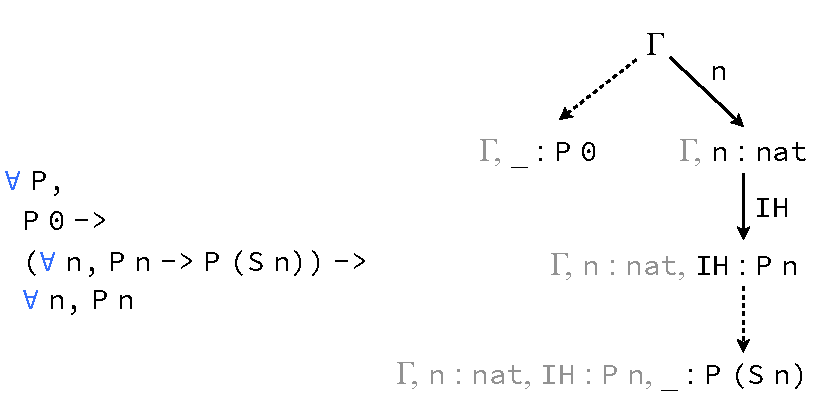
\includegraphics[scale=0.55]{repair/nat_ind}
\end{center}
\caption{The type of (left) and tree for (right) the induction principle \lstinline{nat_ind}. The solid edges represent hypotheses, and the dotted edges represent the proof obligations for each case in an inductive proof.}
\label{fig:cattree}
\end{figure}

\subsubsection{Transformations}

\paragraph{Patch Specialization} Specialization (\lstinline{specialize.ml}) takes a patch candidate and some arguments,
all of which are Coq terms.
It applies the candidate to the arguments, then it $\beta\iota$-reduces~\cite{equality} the result using Coq's
\lstinline{Reduction.nf_betaiota} function. It is the job of the 
patch finding procedure to provide both the candidate and the arguments.

\paragraph{Patch Abstraction} Abstraction (\lstinline{abstraction.ml}) takes a patch candidate, 
the goal type, and the function arguments or function to abstract.
It first generalizes the candidate, wrapping it inside of a lambda from the type of the term to abstract.
Then, it substitutes terms inside the body with the abstract term.
It continues to do this until there is nothing left to abstract, then filters results by the goal type.
Consider, for example, abstracting this candidate by \lstinline{m}:

\begin{lstlisting}[language=coq]
  fun (H : n <= m) => le_plus_trans n m 1 H(@\vspace{-0.04cm}@)
  : n <= m -> n <= m + 1
\end{lstlisting}
The generalization step wraps this in a lambda from some \lstinline{nat}, the type of \lstinline{m}:

\begin{lstlisting}[language=coq]
  fun ((@\diff{n0}@) : nat) =>(@\vspace{-0.04cm}@)
    (fun (H : n <= m) => le_plus_trans n m 1 H)(@\vspace{-0.04cm}@)
  : (@\ltacforall@) (@\diff{n0}@), n <= m -> n <= m + 1
\end{lstlisting}
The substitution step replaces \lstinline{m} with \lstinline{n0}:

\begin{lstlisting}[language=coq]
  fun ((@\diff{n0}@) : nat) =>(@\vspace{-0.04cm}@)
    (fun (H : n <= (@\diff{n0}@)) => le_plus_trans n (@\diff{n0}@) 1 H)(@\vspace{-0.04cm}@)
  : (@\ltacforall@) (@\diff{n0}@), n <= (@\diff{n0}@) -> n <= (@\diff{n0}@) + 1
\end{lstlisting}

Abstraction uses a list of \textit{abstraction strategies} to determine what subterms
to substitute. In this case, the simplest strategy works: The tool
replaces all terms that are convertible to the concrete argument \lstinline{m} with the abstract argument
\lstinline{n0}, which produces a single candidate. Type-checking this candidate confirms that it is a patch.

In some cases, the simplest strategy is not sufficient, even when it is possible to abstract the term.
It may be possible to produce a patch only by abstracting \emph{some} of the subterms
convertible to the argument or function (we show an example of this in Section~\ref{sec:fail}),
or the term may not contain any subterms convertible to the argument or function at all.
We implement several strategies to account for this. The combinations strategy, for example,
tries all combinations of substituting only some of the convertible subterms with the abstract argument. 
The pattern-based strategy substitutes subterms that match a certain pattern
with a term that corresponds to that pattern.

It is the job of the patch finding procedure to provide the candidate and the terms to abstract.
In addition, each configuration includes a list of strategies.
The configuration for changes in conclusions, for example, starts with the simplest strategy,
and moves on to more complex strategies only if that strategy fails.
This design makes abstraction simple to extend with new strategies and simple to call with different strategies
for different classes of changes.

\paragraph{Patch Inversion} Patch inversion (\lstinline{inverting.ml}) exploits symmetry to try to reverse the conclusions of a 
candidate patch.
It first factors the candidate using the factoring component, then calls the primitive inversion
function on each factor, then finally folds the resulting list in reverse.
The primitive inversion function exploits symmetry. 
For example, equality is symmetric, so the component can invert any application of \lstinline{eq_ind} or \lstinline{eq_ind_r}
(any rewrite). Indeed, \lstinline{eq_ind} and \lstinline{eq_ind_r} are inverses, and are related by symmetry:

\begin{lstlisting}[language=coq]
  (@\diff{eq\_ind\_r}@) A x P (H : P x) y (H0 : y = x) :=(@\vspace{-0.04cm}@)
    (@\diff{eq\_ind}@) x (fun y0 : A => P y0) H y ((@\diff{eq\_sym}@) H0)	
\end{lstlisting}
If inversion does not recognize that the type is symmetric, it
swaps subterms and type-checks the result to see if it is an inverse.

\paragraph{Lemma Factoring} The lemma factoring component (\lstinline{factoring.ml}) searches within a term
for its factors. For example,
if the term composes two functions, it returns both factors:

\begin{lstlisting}[language=coq]
  t : (@\diff{X}@) -> (@\diff{Z}@)                (* term *)(@\vspace{-0.04cm}@)
 [f : (@\diff{X}@) -> (@\diff{Y}@); g : (@\diff{Y}@) -> (@\diff{Z}@)] (* factors *)
\end{lstlisting}
In this case, the component takes the composite term and \lstinline{X} as arguments.
It first searches as deep as possible for a term of type \lstinline{X -> Y} for some \lstinline{Y}.
If it finds such a term, then it recursively searches for a term with type \lstinline{Y -> Z}. 
It maintains all possible 
paths of factors along the way, and it discards any paths that cannot reach \lstinline{Z}.

The current implementation can handle paths
with more than two factors, but it fails when \lstinline{Y} depends on \lstinline{X}.
Other components may benefit from dependent factoring; we leave this to future work.

\subsubsection{Inside the Procedure}
\label{sec:algimpl}

The implementation (\lstinline{patcher.ml4}) of the procedure from Section~\ref{sec:composeintro} starts with a
preprocessing step which compiles the proof terms to trees (like the tree in Figure~\ref{fig:cattree}).
It then searches for candidates one step at a time, expanding the trees when necessary.

The \sysname prototype exposes the patch finding procedure to users through the Coq 
command \lstinline{Patch Proof}. \sysname automatically
infers which configuration to use for the procedure from the example change. For example, to
find a patch for the case study in Section~\ref{sec:compcert}, we
used this command:

\begin{lstlisting}[language=ml4]
  Patch Proof Old.unsigned_range unsigned_range as patch.
\end{lstlisting}
\sysname analyzed both versions of \lstinline{unsigned_range} and determined 
that a constructor of the \lstinline{int} type changed (Figure~\ref{fig:int}),
so it initialized the configuration for changes in constructors.

Internally, \sysname represents configurations as sets of options,
which it passes to the procedure. The procedure uses these options to determine
how to compose components (for example, whether to abstract candidates) 
and how to customize components (for example, whether semantic differencing should look for an intermediate lemma).
To implement new configurations for different classes of changes, we simply tweak the options.

\subsection{Workflow Integration}

Needed: hints and so on, any work done since, the Git interface, whatever.

\subsubsection{Trusted Computing Base}
\label{sec:tcb}

A common concern for Coq plugins is an increase in the trusted computing base.
The Coq developers provide a safe plugin API in Coq 8.7 to address this~\cite{coq87news}.
Our prototype takes this into consideration:
While \sysname does not yet support Coq 8.7, it only calls the internal Coq functions that the 
developers plan to expose in the safe API~\cite{coqPR}.
Furthermore, Coq type-checks terms that plugins produce.
Since \sysname does not modify the type checker, it cannot produce an ill-typed term.


\section{Case Study}
\label{sec:case}

We used \toolnameb to automatically discover and lift along ornaments for two scenarios:

\begin{enumerate}
\item Single Iteration: from binary trees to sized binary trees
\item Multiple Iterations: from binary trees to binary search trees to AVL trees
\end{enumerate}

For comparison, we also used the ornaments that \toolnameb discovered to lift functions
and proofs using \textit{Equivalences for Free!}~\cite{tabareau2017equivalences} (EFF),
a more general framework for lifting across equivalences.
\toolnameb produced faster functions and smaller terms, especially when composing multiple iterations of lifting.
In addition, \toolnameb imposed little burden on the user, and the ornaments \toolnameb discovered proved useful to EFF.

We chose EFF for comparison because \toolnameb is the only tool for ornaments in Coq,
and because doing so demonstrates the benefits of specialized automation
for ornaments. \toolnameb can handle only a small class of equivalences
compared to EFF, and it can currently handle only incremental changes to types (one new index at a time).
Our experiences suggest that it is possible to use both tools in concert.
Section~\ref{sec:related} discusses EFF in more detail.

\subparagraph*{Setup.}
The case study code is in the \href{http://github.com/uwplse/ornamental-search/tree/itp+equiv/plugin/eval}{\lstinline{eval}} folder of the repository.
For each scenario,
we ran \toolnameb to search for an ornament,
and then lifted functions and proofs along that ornament using both \toolnameb and EFF.
We noted the amount of user interaction (Section~\ref{sec:caseuser}),
as well as the performance of lifted terms (Section~\ref{sec:caseperf}).
To test the performance of lifted terms, we tested runtime by 
taking the median of ten runs using \lstinline{Time Eval vm_compute} with test values in Coq 8.8.0,
and we tested size by normalizing and running \lstinline{coqwc} on the result.\footnote{i5-5300U, at 2.30GHz, 16 GB RAM}

In the first scenario, we lifted traversal functions along with proofs that their outputs are permutations of each other
from binary trees (\lstinline{tree}) to sized binary trees (\lstinline{Sized.tree}).
In the second scenario, we lifted the traversal functions to AVL trees (\lstinline{avl}) through four intermediate
types (one for each new index),
and we lifted a search function from BSTs (\lstinline{bst}) to AVL trees through
one intermediate type. 
Both scenarios considered only full binary trees.

To fit \lstinline{bst} and \lstinline{avl} into algebraic ornaments for \toolnameb,
we used boolean indices to track invariants.
While the resulting types are not the most natural definitions,
this scenario demonstrates that it is possible to express interesting changes to structured types as algebraic ornaments,
and that lifting across these types in \toolnameb produces efficient functions.

\subsection{User Experience}
\label{sec:caseuser}

For each intermediate type in each scenario, we used \toolnameb to 
discover the components of the equivalence.
These components
were enough for \toolnameb to lift functions and proofs 
with no additional proof burden and no additional axioms.
To use EFF, we also had to prove that these components form an equivalence;
we set the appropriate option to generate these proofs using \toolnameb.
In addition, to use EFF, we had to prove univalent parametricity of each inductive type;
these proofs were small, but required specialized knowledge.
To lift the proof of the theorem \lstinline{pre_permutes} using EFF, 
we had to prove the univalent parametric relation between the unlifted and lifted versions of the
functions that the theorem referenced; this pulled in the functional extensionality axiom, which was not necessary 
using \toolnameb.

In the second scenario, to simulate the incremental workflow \toolnameb requires, we lifted to each intermediate type, then unpacked the result.
For example, the ornament from \lstinline{bst} to \lstinline{avl} passed through an intermediate type;
we lifted \lstinline{search} to this type first, unpacked the result, and then repeated this process.
In this scenario, using EFF differently could have saved some work relative to \toolnameb, since with EFF, it is possible to skip 
the intermediate type;\footnote{The performances of the terms that EFF produces are sensitive to the equivalence used;
for a 100 node tree, this alternate workflow produced a search function
which is hundreds of times slower and traversal functions which are thousands of times slower
than the functions that \toolnameb produced. In addition, the lifted proof of \lstinline{pre_permutes} using EFF failed to normalize
with a timeout of one hour.}
\toolnameb is best fit where an incremental workflow is desirable.

\subsection{Performance}
\label{sec:caseperf}


\begin{figure}
\small
\centering
\resizebox{\columnwidth}{!}{%
\begin{tabular}{ |l|l|c|c|c|c|c| }
 \hline
  & & \textbf{10} & \textbf{100} & \textbf{1000} & \textbf{10000} & \textbf{100000} \\
\hline
 \multirow{3}{*}{\smallmath{$\texttt{preorder}$}} & \textbf{Unlifted} &  $\phantom{1}0.0$ & $\phantom{6}0.0$ & $\phantom{20}0.0\ \phantom{(33.50\mathrm{x})}$ & $\phantom{313}3.0\ \phantom{42}(1.00\mathrm{x})$ & $\phantom{555}37.0\ \phantom{523}(1.00\mathrm{x})$ \\
\cline{2-7}
 & \textbf{\toolnameb} & $\phantom{2}0.0$ & $\phantom{6}0.0$ & $\phantom{33}0.0\ \phantom{(33.50\mathrm{x})}$ & $\phantom{222}3.0\ \phantom{12}(1.00\mathrm{x})$ & $\phantom{513}35.0\ \phantom{522}(0.95\mathrm{x})$ \\
\cline{2-7}
 & \textbf{EFF} & $\phantom{2}0.0$ & $\phantom{6}1.0$ & $\phantom{3}27.0\ \phantom{(33.50\mathrm{x})}$ & $\phantom{2}486.5\ (162.17\mathrm{x})$ & $\phantom{5}8078.5\ \phantom{5}(218.33\mathrm{x})$ \\
\hline
\end{tabular}
}%
%\end{minipage}
\vspace{-0.25cm}
\caption{Median runtime (ms) of unlifted (\lstinline{tree}) and lifted (\lstinline{Sized.tree}) \lstinline{preorder} over ten runs with test inputs ranging from about 10 to about 10000 nodes.}
\label{tab:size1}
\end{figure}

\begin{figure}
\small
\resizebox{\columnwidth}{!}{%
\begin{tabular}{ |l|l|c|c|c|c|c| }
 \hline
   & & \textbf{10} & \textbf{100} & \textbf{1000} & \textbf{10000} & \textbf{100000} \\
\hline
 \multirow{3}{*}{\smallmath{$\texttt{preorder}$}} & \textbf{Unlifted} &  $\phantom{1}0.0$ & $\phantom{6}0.0$ & $\phantom{20}0.0\ \phantom{(33.50\mathrm{x})}$ & $\phantom{313}3.0\ \phantom{42}(1.00\mathrm{x})$ & $\phantom{555}37.0\ \phantom{512}(1.00\mathrm{x})$  \\ \cline{2-7}
 & \textbf{\toolnameb} & $71.5$ & $71.0$ & $\phantom{1}69.0\ \phantom{(33.50\mathrm{x})}$ & $\phantom{12}75.0\ \phantom{4}(25.00\mathrm{x})$ & $\phantom{25}109.0\ \phantom{513}(2.95\mathrm{x})$ \\ \cline{2-7}
 & \textbf{EFF} & $\phantom{1}1.0$ & $11.0$ & $152.0\ \phantom{(33.50\mathrm{x})}$ & $2976.5\ (992.17\mathrm{x})$ & $56636.5\ (1530.72\mathrm{x})$ \\ \hline
 \multirow{3}{*}{\smallmath{$\texttt{search}$}} & \textbf{Unlifted} & $\phantom{1}0.0$ & $\phantom{6}0.0$  & $\phantom{22}2.0\ \phantom{1}(1.00\mathrm{x})$  & $\phantom{123}3.0\ \phantom{42}(1.00\mathrm{x})$ & $\phantom{312}29.0\ \phantom{513}(1.00\mathrm{x})$ \\ \cline{2-7}
 & \textbf{\toolnameb} & $12.0$ & $14.0$ & $\phantom{1}12.0\ \phantom{1}(6.00\mathrm{x})$  & $\phantom{12}15.0\ \phantom{45}(5.00\mathrm{x})$ & $\phantom{512}50.0\ \phantom{555}(1.72\mathrm{x})$ \\ \cline{2-7}
 & \textbf{EFF} & $\phantom{1}1.0$ & $\phantom{6}5.0$ & $\phantom{1}67.0\ (33.50\mathrm{x})$ & $1062.0\ (354.00\mathrm{x})$ & $15370.5\ \phantom{5}(530.02\mathrm{x})$  \\
\hline
\end{tabular}
}
%\end{minipage}
\vspace{-0.25cm}
\caption{Median runtime (ms) of unlifted (\lstinline{tree}) and lifted (\lstinline{avl}) \lstinline{preorder},
plus unlifted (\lstinline{bst}) and lifted (\lstinline{avl}) \lstinline{search}, over ten runs with inputs ranging from about 10 to about 100000 nodes.}
\label{tab:size2}
\end{figure}

Relative to EFF, \toolnameb produced faster functions.
Figure~\ref{tab:size1} summarizes
runtime in the first scenario for \lstinline{preorder},
and Figure~\ref{tab:size2} summarizes
runtime in the second scenario for \lstinline{preorder} and \lstinline{search}.
The \lstinline{inorder} and \lstinline{postorder} functions performed similarly to \lstinline{preorder}.
The functions \toolnameb produced imposed modest overhead for smaller inputs, but were
tens to hundreds of times faster than the functions that EFF produced for larger inputs.
This performance gap was more pronounced over multiple iterations of lifting.

\toolnameb also produced smaller terms:
in the first scenario, 13 vs. 25 LOC for \lstinline{preorder},
12 vs. 24 LOC for \lstinline{inorder}, and 17 vs. 29 LOC for \lstinline{postorder};
and in the second scenario, 21 vs. 120 LOC for \lstinline{preorder}, 20 vs. 119 LOC for \lstinline{inorder}, 
24 vs. 125 LOC for \lstinline{postorder}, and 31 vs. 52 LOC for \lstinline{search}.
In the first scenario, the lifted proof of \lstinline{pre_permutes} using \toolnameb was 85 LOC;
the lifted proof of \lstinline{pre_permutes} using EFF was 1463184 LOC.

We suspect \toolnameb provided these performance benefits because it directly
lifted induction principles, whereas EFF produced lifted functions in terms of unlifted functions. 
The multiple iteration case in particular highlights this,
since EFF's approach makes lifted terms much slower and larger as the number of iterations increases,
while \toolnameb's approach does not.



\chapter{Related Work}

% TODO whatever else isn't here yet, and some of this might be factored out or partially factored out---all papers, including survey, plus generals

\section{Programs}

\subsection*{Program Refactoring} 

Refactoring~\cite{Mens:2004:SSR:972215.972286}.

\subsection*{Program Repair} 

% From PUMPKIN PATCH, unchanged

Adapting proofs to changes is essentially program repair
for dependently typed languages. 
Program repair tools for 
languages with non-dependent type 
systems~\cite{Pei:2014:APR:2731750.2731779, Long:2016:APG:2837614.2837617, Le:2017:SSS:3106237.3106309, Mechtaev:2016:ASM:2884781.2884807, Monperrus2015} 
may have applications in the context of a dependently typed language.
Similarly, our work may have applications within program repair in these languages:
Future applications of our approach may repurpose it to repair programs for functional languages.

\subsection*{Ornaments}

% From PUMPKIN PATCH, unchanged

Ornaments~\cite{Dagand17jfp, Williams:2014:OP:2633628.2633631}
separate the computational and logical components of a datatype, and may
make proofs more resilient to datatype changes.

\subsection*{Programming by Example}

% From PUMPKIN PATCH, unchanged

Our approach generalizes an example that the programmer provides.
This is similar to programming by example, a subfield of 
program synthesis~\cite{DBLP:journals/ftpl/GulwaniPS17}. 
This field addresses different challenges in different logics,
but may drive solutions to similar problems in a dependently typed language.

\subsection*{Differencing \& Incremental Computation}

% From PUMPKIN PATCH, unchanged

Existing work in differencing and incremental computation may help 
improve our semantic differencing component.
Type-directed diffing~\cite{Miraldo:2017:TDS:3122975.3122976}
finds differences in algebraic data types.
Semantics-based change impact analysis~\cite{Autexier:2010:SCI:1860559.1860580} models semantic differences
between documents.
Differential assertion checking~\cite{differential-assertion-checking-2} analyzes different
versions of a program for relative correctness with respect to a specification.
Incremental $\lambda$-calculus~\cite{Cai:2014:TCH:2594291.2594304} introduces a general model for program changes.
All of these may be useful for improving semantic differencing.

\section{Proofs}

\subsection*{Proof Reuse}

% From PUMPKIN PATCH, unchanged

Our approach reimagines the problem of proof reuse in the context of proof automation.
While we focus on changes that occur over time, traditional proof reuse techniques can help
improve our approach.
Existing work in proof reuse focuses on transferring proofs between isomorphisms,
either through extending the type system~\cite{Barthe:2001:TIP:646793.704711} or through an automatic method~\cite{Magaud2002}.
This is later generalized and implemented in Isabelle~\cite{Huffman2013} and Coq~\cite{ZimmermannH15, tabareau:hal-01559073};
later methods can also handle implications. 
%Transfer tactics apply these functions but do not infer them, while our approach
%infers these functions but does not apply them.
Integrating a transfer tactic with a proof patch finding tool will create an end-to-end
tool that can both find patches and apply them automatically.

Proof reuse for extended inductive types~\cite{Boite2004} adapts proof obligations
to structural changes in inductive types. Later work~\cite{Mulhern06proofweaving} proposes a method
to generate proofs for new constructors. These approaches may be useful when extending the differencing
component to handle structural changes. Existing work in theorem reuse and proof generalization~\cite{Felty1994, pons00, Johnsen2004} abstracts existing proofs for reusability, and may be useful
for improving the abstraction component.
Our work focuses on the components critical to searching for patches; these complementary approaches
can drive improvements to the components.

\subsection*{Proof Evolution}

% From PUMPKIN PATCH, unchanged

There is a small body of work on change and dependency management for verification,
both to evaluate impact of potential changes and maximize reuse~\cite{873647, Autexier:2010:CMH:1986659.1986663}
and to optimize build performance~\cite{Celik:2017:IRP:3155562.3155588}.
These approaches may help isolate changes, which is necessary to identify future benchmarks, integrate
with CI systems, and fully support version updates.

\subsection*{Proof Refactoring}

\subsection*{Proof Repair}

\subsection*{Proof Design}

% From PUMPKIN PATCH, unchanged:

Existing proof engineering work addresses brittleness
by planning for changes~\cite{proof-eng} and designing theorems and proofs that make maintenance less of an issue.
Design principles for specific domains (such as formal metatheory~\cite{Aydemir2008, Delaware2013POPL, Delaware2013ICFP})
can make verification more tractable. CertiKOS~\cite{certikos} introduces the idea of a deep specification to
ease verification of large systems.
These design principles and frameworks are complementary to our approach.
Even when programmers use informed design principles,
changes outside of the programmer's control can break proofs;
our approach addresses these changes.

\subsection*{Proof Automation}

% From PUMPKIN PATCH, unchanged:

We address a missed opportunity in proof automation for ITP: searching
for patches that can fix broken proofs.
This is complementary to existing automation techniques. Nonetheless, there is a wealth
of work in proof automation that makes proofs more resilient to change.
Powerful tactics like \lstinline{crush}~\cite{chlipala:cpdt} can make
proofs more resilient to changes. 
Hammers like Isabelle's sledgehammer~\cite{Blanchette2013} can make proofs agnostic to some low-level changes.
Recent work~\cite{coqhammer} paves the way for a hammer in Coq.
Even the most powerful tactics cannot address all changes;
our hope is to open more possibilities for automation.

Powerful project-specific tactics~\cite{chlipala:cpdt, Chlipala2013} can help prevent low-level maintenance tasks.
Writing these tactics requires good engineering~\cite{Gonthier2011} and domain-specific knowledge,
and these tactics still sometimes break in the face of change.
A future patching tool may be able to repair tactics; the debugging process
for adapting a tactic is not too dissimilar to providing an example to a tool.

Rippling~\cite{rippling} is a technique for automating inductive proofs that uses restricted rewrite rules to
guide the inductive hypothesis toward the conclusion; this may guide improvements to the
differencing, abstraction, and specialization components.
The abstraction and factoring components address specific classes of unification problems;
recent developments to higher-order unification~\cite{Miller:2012:PHL:2331097} may help
improve these components.
Lean~\cite{selsam:lean} introduces the first congruence closure algorithm for dependent type theory that
relies only on the Uniqueness of Identity Proofs (UIP) axiom. While UIP is not fundamental to Coq,
it is frequently assumed as an axiom; when it is, it may be tractable to use a similar algorithm to improve the tool.

GALILEO~\cite{bundyreasoning} repairs faulty physics theories
in the context of a classical higher-order logic (HOL); there is preliminary work extending this
style of repair to mathematical proofs. 
Knowledge-sharing methods~\cite{tgck-cicm14} can adapt some proofs across different representations of HOL.
These complementary approaches may guide extensions to support decidable domains and classical logics.

\subsection*{Transport}

\subsection*{Parametricity}

\subsection*{Refinement}



\section{Conclusions \& Future Work}
\label{sec:concl}

We presented \toolnameb: a tool for searching for and lifting across algebraic ornaments in Coq.
\toolnameb is the first tool to lift across ornaments in a non-embedded dependently typed language,
and to automatically infer certain kinds of ornaments from types alone.
Our algorithms give efficient transport across equivalences arising
from algebraic ornaments; our case study demonstrates that such automation can make lifted
terms smaller and faster as part of an incremental workflow.

\subparagraph*{Future Work.} 
A future version may support other ornaments beyond algebraic ornaments,
with additional user interaction as needed; this may help support, for example,
the ornament between \lstinline{nat} and \lstinline{list}, where \lstinline{list}
has a new element in the \lstinline{cons} case.
A future version may loosen restrictions on input types to support
adding constructors while preserving inductive structure, recursive references under products,
and coinductive types. Integrating with \textsc{Pumpkin Patch}~\cite{ringer2018adapting} 
may help remove restrictions \toolnameb makes about the hypotheses of \B.
\lstinline{Preprocess} currently supports only certain fixpoints;
a more general translation may help \toolnameb support more terms, and discussions
with Coq developers suggest that the implementation of such a translation
building on work from the equations~\cite{sozeau:equations} plugin is in progress.
Extending \toolnameb to generate proofs of coherence conditions for lifted terms may increase user confidence.
Proofs that the commands that \toolnameb implements satisfy their specifications may also increase user confidence.
Better automating the recovery of user-friendly types may improve user experience.



%\begin{acks}

%We thank Valentin Robert and Zach Tatlock for valuable conversations about proof patching.
%We thank Leonardo de Moura and the UW PLSE lab for helpful suggestions.
%We thank the students and lecturers from the first DeepSpec Summer School for motivating future work.
%We thank Dan Licata for pointers in understanding the mathematical properties of inductive types.
%This material is based upon work supported by the National Science Foundation Graduate Research Fellowship under Grant No. DGE-1256082.
%Any opinions, findings, and conclusions or recommendations expressed in this material are those of the 
%authors and do not necessarily reflect the views of the National Science Foundation.

%\end{acks}



\bibliography{ornbib}

\end{document}
